\chapter{传播效应：等离子体、尘埃与引力透镜}
\label{chap:e21}

\begin{chapteropening}
到现在为止，我们几乎都在问同一类问题：\textbf{源本来是什么样子？}——它的角直径、它的相干时间、它的光子统计。可是有一件事我们一直偷偷假设掉了：光从源出发，一路飞到望远镜，中间那几千光年、几十亿光年，是"透明"的。它当然不是。光要穿过稀薄的自由电子、湍动的磁化等离子体、飘着尘埃颗粒的星云、乃至被大质量天体压弯的时空。每穿过一层，它的到达时间、频率、偏振、方向、甚至"有几个副本"都会被悄悄改写。

本章要把这条"路上发生了什么"讲清楚。主线是：先把传播看成一条\textbf{有记忆的通道}（channel with memory）——它不是简单地把信号乘一个常数，而是把每个光子身上的标签重新填一遍。然后我们逐个拆开四类改写者：冷等离子体的\(\nu^{-2}\)色散（我们会一步不跳地推出"为什么低频光子迟到"）、湍流带来的散射与闪烁、尘埃的消光与红化、以及弯曲时空的引力透镜。最后回到本书的老本行：这些效应既\textbf{污染}信号（把相干性抹平、把时间戳拖乱），也\textbf{编码}信号（在色散量里存下电子账本，在时间延迟里存下宇宙学）。它承接第 \ref{chap:e02} 章的带宽与相干时间、第 \ref{chap:e13} 章的时间同步，是把"源端物理"翻译成"探测器事件"的最后一道工序。
\end{chapteropening}

\section{把传播当成一条有记忆的通道}
\label{sec:e21-channel}

先建立画面。最省事的想法是把介质当成一块灰玻璃：光穿过去，暗了一点、红了一点，其余不变。对求平均亮度、平均颜色，这个"乘一个常数"的图像有时够用。但本书关心的是\textbf{事件表}（第 \ref{chap:e13} 章）——每个光子候选带着到达时刻、频率、偏振、方向这几个标签；也关心\textbf{相干性}——不同时刻、不同望远镜之间场的相位关系。对这些量，"灰玻璃"是灾难性的近似，因为传播真正做的事是\textbf{把标签重写}：频率标签决定它迟到多少，偏振标签会被磁场旋转，方向标签被散射打散、被透镜复制，到达时间标签会被多条路径拖出回声。

所以更好的第一步不是问"源本来多亮"，而是问"源端的场要经过怎样一条通道，才变成我探测器上的一次事件"。把它写成线性通道最直接。在时间域里，第 \(i\) 个观测通道（某个偏振、某台望远镜、某个像、某个频道）的电场是源端各通道场的\textbf{卷积叠加}：
\begin{equation}
  E_{{\rm out},i}(t)
  =
  \sum_j\int h_{ij}(t-t')\,E_{{\rm src},j}(t')\,{\rm d}t'
  + n_i(t) .
  \label{eq:e21-channel-time}
\end{equation}
\begin{formulaexplain}
\(E_{{\rm out},i}\) 是第 \(i\) 个观测通道的场，\(E_{{\rm src},j}\) 是第 \(j\) 个源端通道的场，\(h_{ij}\) 是从 \(j\) 到 \(i\) 的响应函数，\(n_i\) 是前景与探测噪声。积分号是关键：传播\textbf{有记忆}——一个源端时刻的光会被延迟、展宽后贡献到许多观测时刻。
\end{formulaexplain}
逐个符号说清楚：\(i,j\) 标记偏振、望远镜、像或频道（无量纲编号）；\(h_{ij}(t-t')\) 是脉冲响应（impulse response），它的量纲取决于场的归一化，但真正用得上的是它的三个特征——\textbf{时间宽度}（信号被展宽多少）、\textbf{峰值延迟}（信号整体迟到多少）、以及不同通道之间的\textbf{相对相位}；\(n_i(t)\) 是前景热辐射、天光背景和探测链噪声之和。如果介质只吸收不散射，\(h_{ij}\) 近似是个对角的、被压低了幅度的 delta 函数；如果有 Faraday 旋转，它会在两个线偏振通道之间"转账"；如果有散射或透镜，它同时把方向和到达时间搅在一起。地球质心改正、钟差、大气延迟、仪器电子延迟，也都是这个 \(h_{ij}\) 的一部分——脉冲星计时（pulsar timing）正是把这些项一项项拆到纳秒量级的最成熟范例 \citep{2006MNRAS.372.1549E}。

翻回事件表的语言：一个光子候选是一行 \((t_q,\nu_q,p_q,\bm{x}_q,w_q)\)——到达时刻 \(t_q\)（单位 s）、频率 \(\nu_q\)（单位 Hz）、偏振通道 \(p_q\)、空间标签 \(\bm{x}_q\)（像素、基线或望远镜编号）、质量权重 \(w_q\)。这一节剩下要做的，就是把式 \eqref{eq:e21-channel-time} 那个抽象的 \(h_{ij}\)，对四类介质各写出一个具体形式，看它到底怎么改这五个标签：色散改 \(t_q(\nu_q)\)，Faraday 旋转改 \(p_q(\lambda_q^2)\)，散射把一个窄脉冲的 \(t_q\) 摊成一条长尾，尘埃改不同 \(\lambda_q\) 被接收的概率，透镜把一个源事件复制成好几组 \((\bm{x}_q,t_q)\)。

在开始之前，先把\textbf{数量级的地图}摊在桌上，这样后面每算一个数字都知道自己站在哪。银河系高银纬方向的色散量（我们马上会定义）常在 \(30\text{--}100\,{\rm pc\,cm^{-3}}\)，而快速射电暴（fast radio burst，FRB）能到 \(10^{3}\text{--}10^{4}\,{\rm pc\,cm^{-3}}\)。普通星际介质的旋转量多为 \(1\text{--}10^{2}\,{\rm rad\,m^{-2}}\)，强磁化致密环境可到 \(10^{4}\text{--}10^{5}\,{\rm rad\,m^{-2}}\)。散射展宽从微秒到秒，低频端涨得极快。光学消光在高银纬常小于 \(0.1\) 星等，在银盘和分子云里能到好几星等。引力透镜的时间延迟跨度最大：恒星质量透镜在微秒到毫秒，星系强透镜常在天到年。记住这张地图，本章的每一条公式都能落在一个真实的数字上。

\section{冷等离子体色散：为什么低频光子迟到}
\label{sec:e21-dispersion}

先挑最干净的一位改写者：冷等离子体（cold plasma），也就是弥漫在星际、星系际空间里的稀薄自由电子。它有一个非常温和又非常有用的性质：它不会把脉冲随机化，只是让\textbf{低频光子稍微迟到}。而"迟到多少"精确正比于一路上遇到的电子总数。这就是说，色散既是"污染"（它把一个瞬间的爆发在频率上抹成一道扫频的斜线），又是"编码"（那道斜线的斜率，就是视线方向的电子账本）。我们把这条 \(\nu^{-2}\) 定律一步不跳地推出来。

\paragraph{从折射率到群速度}
\label{sec:e21-groupvel}

自由电子对电磁波的响应，给出冷等离子体的折射率。当波频远高于等离子体频率时（我们稍后验证这个条件对射电观测成立），
\begin{equation}
  n(\omega)\simeq 1-\frac{\omega_p^2}{2\omega^2},
  \qquad
  \omega_p^2=\frac{4\pi n_e e^2}{m_e}.
  \label{eq:e21-plasma-index}
\end{equation}
\begin{formulaexplain}
\(n(\omega)\) 是折射率（无量纲），\(\omega\) 是角频率，\(\omega_p\) 是等离子体频率，\(n_e\) 是自由电子数密度，\(e,m_e\) 是电子电荷与质量（CGS 单位）。电子越多，\(\omega_p\) 越大，低频波偏离真空传播就越明显。
\end{formulaexplain}
逐个符号落地：\(n_e\) 单位是 \({\rm cm^{-3}}\)，银河系温暖电离介质常为 \(10^{-2}\text{--}10^{-1}\,{\rm cm^{-3}}\)，HII 区和 FRB 的宿主环境可高很多个数量级；\(\omega_p=\sqrt{4\pi n_e e^2/m_e}\) 是等离子体自身的固有振荡频率（单位 \({\rm rad\,s^{-1}}\)）。代个数感受一下：取 \(n_e=0.03\,{\rm cm^{-3}}\)，用 CGS 值 \(e=4.8\times10^{-10}\,{\rm esu}\)、\(m_e=9.1\times10^{-28}\,{\rm g}\)，得 \(\omega_p\approx 9.8\times10^{3}\,{\rm rad\,s^{-1}}\)，对应频率 \(\nu_p=\omega_p/2\pi\approx1.5\,{\rm kHz}\)。而射电观测在 \(\nu\sim10^{8}\text{--}10^{9}\,{\rm Hz}\)，所以 \(\omega\gg\omega_p\) 成立得极其充分，式 \eqref{eq:e21-plasma-index} 里对 \(\omega_p^2/\omega^2\) 只保留到一阶完全够用。

关键的物理是：信息（脉冲包络）不以相速度传播，而以\textbf{群速度}（group velocity）\(v_g={\rm d}\omega/{\rm d}k\) 传播——这是第 \ref{chap:e02} 章讲波包时就强调过的。要算 \(v_g\)，先写色散关系 \(k=n\omega/c\)：
\[
  k=\frac{n\omega}{c}
   =\frac{\omega}{c}\left(1-\frac{\omega_p^2}{2\omega^2}\right)
   =\frac{\omega}{c}-\frac{\omega_p^2}{2c\,\omega}.
\]
逐项对 \(\omega\) 求导（第二项用 \({\rm d}(\omega^{-1})/{\rm d}\omega=-\omega^{-2}\)）：
\[
  \frac{{\rm d}k}{{\rm d}\omega}
  =\frac{1}{c}-\frac{\omega_p^2}{2c}\cdot\left(-\frac{1}{\omega^2}\right)
  =\frac{1}{c}\left(1+\frac{\omega_p^2}{2\omega^2}\right).
\]
群速度就是它的倒数，再用几何级数 \((1+x)^{-1}\approx1-x\)（因为 \(x=\omega_p^2/2\omega^2\ll1\)）展开到一阶：
\[
  v_g=\frac{{\rm d}\omega}{{\rm d}k}
     =\frac{c}{1+\dfrac{\omega_p^2}{2\omega^2}}
     \approx c\left(1-\frac{\omega_p^2}{2\omega^2}\right).
\]
这一步已经能"看见"物理了：\(v_g<c\)，而且\textbf{频率越低（\(\omega\) 越小），\(\omega_p^2/2\omega^2\) 越大，群速度越慢}。慢，就意味着迟到。低频光子迟到的根源，就是这一行。

\paragraph{把迟到时间沿视线累加出来}
\label{sec:e21-dmderive}

现在把"慢"翻译成"迟到多少"。一段路程 \({\rm d}l\) 花的时间是 \({\rm d}l/v_g\)，沿整条视线积分：
\[
  t=\int\frac{{\rm d}l}{v_g}
   =\int\frac{1}{c}\left(1+\frac{\omega_p^2}{2\omega^2}\right){\rm d}l
   =\underbrace{\frac{L}{c}}_{\text{真空飞行}}
   +\underbrace{\frac{1}{2c\,\omega^2}\int\omega_p^2\,{\rm d}l}_{\text{色散附加延迟}} .
\]
第一项是光在真空里飞完全程 \(L\) 的时间，与频率无关，观测上只是一个总的零点，测不出来。真正能测的是第二项——它才是\textbf{频率相关}的迟到。把 \(\omega_p^2=4\pi n_e e^2/m_e\) 代进去，注意 \(4\pi e^2/m_e\) 是常数可以提到积分外：
\[
  \Delta t
  =\frac{1}{2c\,\omega^2}\int\frac{4\pi n_e e^2}{m_e}\,{\rm d}l
  =\frac{2\pi e^2}{m_e c\,\omega^2}\int n_e\,{\rm d}l .
\]
最后用 \(\omega=2\pi\nu\)，即 \(\omega^2=4\pi^2\nu^2\)：
\begin{equation}
  \Delta t
  =\frac{e^2}{2\pi m_e c}\,\frac{1}{\nu^2}\int n_e\,{\rm d}l
  \equiv \frac{e^2}{2\pi m_e c}\,\frac{{\rm DM}}{\nu^2},
  \qquad
  {\rm DM}\equiv\int n_e\,{\rm d}l .
  \label{eq:e21-dm-delay}
\end{equation}
\begin{formulaexplain}
\(\Delta t\) 是相对真空的附加延迟，\(\nu\) 是观测频率，DM 是\textbf{色散量}（dispersion measure），即视线方向自由电子的柱密度 \(\int n_e\,{\rm d}l\)。整条式子的骨架是 \(\Delta t\propto {\rm DM}/\nu^{2}\)：迟到时间正比于一路上的电子总数，反比于频率的平方。
\end{formulaexplain}
这条式子把三件事一次讲清。第一，\(\Delta t\propto\nu^{-2}\)——这就是"低频迟到"的定量版，而且我们是从群速度一路推下来的，没有跳步。第二，前面那坨常数 \(e^2/(2\pi m_e c)\) 是纯物理常数（在 CGS 里）；把 DM 的路径元 \({\rm d}l\) 用天文学惯用的 pc、频率用 GHz 代入，两个频率通道之间的延迟差就是天文学家背得滚瓜烂熟的
\begin{equation}
  \Delta t_{\rm DM}
  =
  4.148808\,{\rm ms}\;
  \frac{{\rm DM}}{{\rm pc\,cm^{-3}}}
  \left[
  \left(\frac{\nu_1}{\rm GHz}\right)^{-2}
  -
  \left(\frac{\nu_2}{\rm GHz}\right)^{-2}
  \right].
  \label{eq:e21-dispersion-delay}
\end{equation}
\begin{formulaexplain}
\(\Delta t_{\rm DM}\) 是频率 \(\nu_1\) 与 \(\nu_2\) 两个通道之间的到达时差。系数 \(4.148808\,{\rm ms}\) 就是把式 \eqref{eq:e21-dm-delay} 的物理常数换成 pc、\({\rm cm^{-3}}\)、GHz 后的数值。低频（\(\nu_1<\nu_2\)）的那一项 \(\nu_1^{-2}\) 更大，所以低频通道迟到，动态谱里看到的就是那道向右下弯的扫频轨迹。
\end{formulaexplain}
第三，DM 是\textbf{柱密度而非局部密度}——它只关心一路上一共有多少电子，不关心它们怎么分布。单位是 \({\rm pc\,cm^{-3}}\)（把长度 pc 和数密度 \({\rm cm^{-3}}\) 相乘）。

代真实数字落地。取 \({\rm DM}=300\,{\rm pc\,cm^{-3}}\)（一颗中等距离脉冲星的典型值），\(\nu_1=0.6\,{\rm GHz}\)、\(\nu_2=1.4\,{\rm GHz}\)：
\[
  \Delta t_{\rm DM}=4.148808\times300\times\left(0.6^{-2}-1.4^{-2}\right)\,{\rm ms}
  \approx 1244.6\times(2.778-0.510)\,{\rm ms}\approx 2822\,{\rm ms}\approx 2.8\,{\rm s}.
\]
将近三秒！同一次爆发，\(0.6\) GHz 的信号比 \(1.4\) GHz 晚到快三秒。正因如此，射电脉冲和 FRB 的搜索要先在一排试探色散量（trial DM）上做\textbf{去色散}（de-dispersion），把每个频道按 \(\nu^{-2}\) 往回平移，直到不同频道的脉冲重新对齐、信噪比冒尖，那个让信噪比最大的 DM 就是测量值。

还有一个容易被忽视的\textbf{污染}：即便整体去色散做对了，每个频率通道本身有有限带宽 \(\Delta\nu\)，通道内部高低频端的延迟差没被补掉，会把脉冲抹宽：
\begin{equation}
  \Delta t_{\rm chan}
  \simeq
  8.3\,\mu{\rm s}\;
  \left(\frac{{\rm DM}}{{\rm pc\,cm^{-3}}}\right)
  \left(\frac{\Delta\nu}{\rm MHz}\right)
  \left(\frac{\nu}{\rm GHz}\right)^{-3}.
  \label{eq:e21-channel-smearing}
\end{equation}
\begin{formulaexplain}
\(\Delta t_{\rm chan}\) 是一个有限带宽通道内部残留的色散展宽，\(\Delta\nu\) 是通道带宽，\(\nu\) 是通道中心频率。它是式 \eqref{eq:e21-dispersion-delay} 对 \(\nu\) 求微分再乘 \(\Delta\nu\) 的结果，所以带 \(\nu^{-3}\)。含义：DM 越高、通道越宽、频率越低，越容易把微秒级的精细结构洗平。
\end{formulaexplain}
它和第 \ref{chap:e02} 章的精神一脉相承：想要好的时间分辨，就得付出带宽的代价，只不过这里的代价是被色散放大的。对高时间分辨天文学，式 \eqref{eq:e21-channel-smearing} 直接决定了通道要切多细。

\begin{figure}[tbp]
\centering
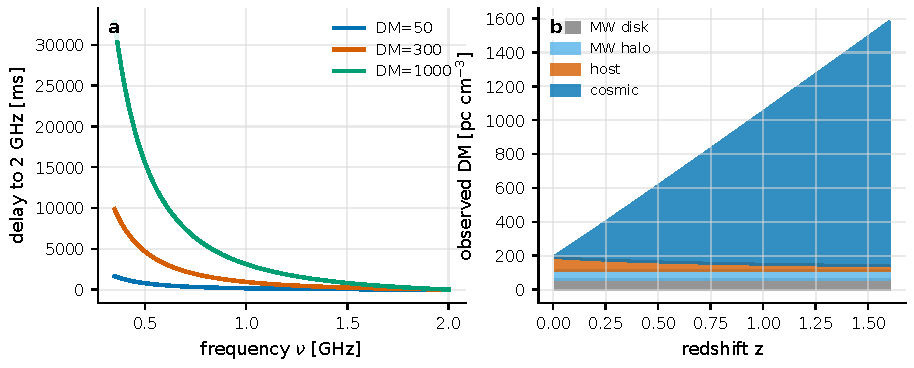
\includegraphics[width=0.94\linewidth]{figures/generated/chapter_14/ch14_dispersion_delay.pdf}
\caption{冷等离子体色散与 FRB 的色散量预算。左图把到达延迟画成频率的函数（参考频率 \(2\,{\rm GHz}\)）：低频端那条陡峭的 \(\nu^{-2}\) 曲线，就是式 \eqref{eq:e21-dispersion-delay} 让 DM 极易从宽带动态谱中读出的原因。右图把一次局域 FRB 的观测色散量拆成银河系盘、银晕、宿主星系与宇宙学等离子体四部分；宿主项因宇宙学时间膨胀按 \((1+z)^{-1}\) 进入观测值。}
\label{fig:e21-dispersion}
\end{figure}

\paragraph{色散量作为电子账本：从银河系到宇宙学}
\label{sec:e21-dmbudget}

既然 DM 是电子账本，就能反过来用它测电子。但账本必须分清是谁欠的。银河系电子密度绝非常数：NE2001 模型把厚盘、薄盘、旋臂、局部空洞和团块拼起来，用脉冲星的 DM、独立测距和散射数据约束参数；YMW16 更新了厚盘、薄盘、旋臂、银心和麦哲伦云/星系际处理，专门把一颗脉冲星或一次 FRB 的\textbf{银河系那部分 DM} 换算成距离或前景 \citep{2002astro.ph..7156C,2017ApJ...835...29Y}。高银纬视线的银河系盘贡献常为 \(30\text{--}100\,{\rm pc\,cm^{-3}}\)，银晕再添 \(50\text{--}100\,{\rm pc\,cm^{-3}}\) 量级；靠近银盘、HII 区或超新星遗迹时，局部结构会比平滑模型更重要。

对宇宙学 FRB，观测到的总色散量是一笔跨越几十亿光年的账：
\begin{equation}
  {\rm DM}_{\rm FRB}
  =
  {\rm DM}_{\rm MW,ISM}
  +{\rm DM}_{\rm MW,halo}
  +{\rm DM}_{\rm cosmic}(z)
  +\frac{{\rm DM}_{\rm host}}{1+z} .
  \label{eq:e21-frb-dm-budget}
\end{equation}
\begin{formulaexplain}
四项分别是银河系盘、银晕、沿途宇宙学等离子体、以及宿主星系的贡献。宿主项要除以 \((1+z)\)，因为宿主处发出的频率间隔和时间间隔在飞往我们的途中已经被宇宙膨胀拉伸了红移倍——同一物理延迟，在我们看来变小了。
\end{formulaexplain}
逐项的物理含义：前两项来自我们自己银河系，可以用 NE2001/YMW16 扣掉；\({\rm DM}_{\rm cosmic}(z)\) 是弥漫在星系际的重子电子，随红移单调增长，是这条式子里最值钱的一项；\({\rm DM}_{\rm host}\) 是宿主星系的贡献，最难约束。把宇宙学项写成均匀宇宙的积分：
\begin{equation}
  {\rm DM}_{\rm cosmic}(z)
  =
  \frac{3cH_0\Omega_b f_{\rm IGM}}{8\pi Gm_p}
  \int_0^z
  \frac{f_e(z')(1+z')}{\sqrt{\Omega_m(1+z')^3+\Omega_\Lambda}}
  \,{\rm d}z' .
  \label{eq:e21-cosmic-dm}
\end{equation}
\begin{formulaexplain}
\(\Omega_b,\Omega_m,\Omega_\Lambda\) 是重子、物质、暗能量密度参数，\(H_0\) 是哈勃常数，\(m_p\) 是质子质量，\(f_{\rm IGM}\) 是进入弥散星系际介质的重子比例，\(f_e\) 是每个重子提供的自由电子数。前面的系数给出平均重子密度，积分核描述膨胀宇宙里电子数密度与路径长度如何随红移变化。
\end{formulaexplain}
这条式子的分量都不神秘：系数 \(3H_0^2\Omega_b/8\pi G\) 是今天的平均重子质量密度（把临界密度乘以 \(\Omega_b\)），除以 \(m_p\) 变成数密度，再乘 \(f_e f_{\rm IGM}\) 得电子数密度；积分里的 \((1+z')\) 来自密度随膨胀的稀释被路径压缩抵消后的净因子，分母的 \(\sqrt{\Omega_m(1+z')^3+\Omega_\Lambda}\) 是 \(\Lambda\)CDM 的膨胀率 \(H(z')/H_0\)。这里有一步千万别漏：视线元不是 \({\rm d}l\) 而是随红移写的 \({\rm d}l=c\,{\rm d}z'/H(z')\)，它单独贡献一个 \(c/H_0\)（\(H_0\) 从 \(H(z')=H_0\sqrt{\cdots}\) 里提出来放进积分核的分母）。正是这个 \(c/H_0\) 和临界密度里的 \(H_0^2\) 合并，才把前因子从"\(3H_0^2\Omega_b/(8\pi G)\) 除以 \(m_p\)"的质量密度形式，凑成式中带 \(cH_0\) 的 \(3cH_0\Omega_b f_{\rm IGM}/(8\pi Gm_p)\)——比纯质量密度多一次 \(c/H_0\)。读者若自己代数，务必记得这一份来自 \({\rm d}l=c\,{\rm d}z'/H(z')\) 的 \(c/H_0\)，否则前因子会差一个因子。它的物理意义惊人地实用：\textbf{FRB 的 DM–红移关系直接称量了宇宙里的重子有多少}——这曾经是"丢失的重子"难题，如今 FRB 样本给出的这条关系已经能测量宇宙重子含量。真实的散布来自宇宙网（cosmic web）的不均匀，常写成 \(\sigma_{\rm DM}\simeq F z^{-1/2}\)，\(F\sim0.1\text{--}0.4\) 对应不同的反馈与晕气体分布 \citep{2020Natur.581..391M,2014ApJ...790..101S}。这是"污染变编码"最漂亮的一例：色散本来是挡在源前面的一层雾，结果这层雾自己称出了宇宙的重子。

\section{Faraday 旋转：给色散加上磁场的方向}
\label{sec:e21-faraday}

色散只数电子的个数，把磁场的信息丢了。如果等离子体是\textbf{磁化}的，还有第二道印记：左旋和右旋圆偏振在磁化等离子体里相速度不同，于是线偏振的振动面会随传播被旋转，且旋转角精确正比于波长平方：
\begin{equation}
  \psi(\lambda)=\psi_0+{\rm RM}\,\lambda^2 .
  \label{eq:e21-rm-angle}
\end{equation}
\begin{formulaexplain}
\(\psi\) 是观测到的线偏振角，\(\psi_0\) 是源的本征偏振角，\(\lambda\) 是波长，RM 是\textbf{旋转量}（rotation measure）。偏振角对 \(\lambda^2\) 的斜率就是 RM。所以只要在几个频率上测偏振角，画成 \(\psi\)–\(\lambda^2\) 图，斜率即得磁化等离子体的累积效应。
\end{formulaexplain}
它和色散是一对姊妹：色散给到达时间一个 \(\nu^{-2}\)（等价于 \(\lambda^2\)）的斜率，Faraday 给偏振角一个 \(\lambda^2\) 的斜率。两者都是"读斜率"。旋转量本身是电子密度与视线磁场分量的路径积分：
\begin{equation}
  {\rm RM}
  =
  0.812
  \int
  \left(\frac{n_e}{{\rm cm^{-3}}}\right)
  \left(\frac{B_\parallel}{\mu{\rm G}}\right)
  \left(\frac{{\rm d}l}{\rm pc}\right)
  \;{\rm rad\,m^{-2}} .
  \label{eq:e21-rm-definition}
\end{equation}
\begin{formulaexplain}
\(B_\parallel\) 是沿视线（指向观测者）的磁场分量，单位微高斯（\(\mu{\rm G}\)）。RM 与 DM 的关键差别：DM 的被积函数是 \(n_e\)（恒正，只会累加），RM 的被积函数是 \(n_e B_\parallel\)（带符号，磁场反向会相互抵消）。所以 RM 携带磁场的\textbf{方向}信息。
\end{formulaexplain}
把两者相除，就得到一个电子加权的视线平均磁场估计：
\begin{equation}
  \langle B_\parallel\rangle
  \simeq
  1.232\,\mu{\rm G}\;
  \frac{{\rm RM}/{\rm rad\,m^{-2}}}{{\rm DM}/{\rm pc\,cm^{-3}}}.
  \label{eq:e21-bfield-rm-dm}
\end{equation}
\begin{formulaexplain}
\(\langle B_\parallel\rangle\) 是由 RM 与 DM 之比推出的平均视线磁场。系数 \(1.232\,\mu{\rm G}\) 就是式 \eqref{eq:e21-rm-definition} 与 DM 定义里两个数值系数的比。只有当 RM 与 DM 来自\textbf{同一段介质}时，这个比值才有直接的物理含义。
\end{formulaexplain}
这不是一个"放之四海皆准"的磁场测量，用它时要盯紧两个陷阱。其一，若 RM 主要来自磁化的宿主星系、而 DM 主要来自星系际介质，两者不是同一段路，式 \eqref{eq:e21-bfield-rm-dm} 会严重低估局部磁场。其二，若视线上磁场有反向，RM 里正负抵消而 DM 不会，比值同样失真。星系团和星系际磁场的 RM 研究，常把这类简并（degeneracy）与 X 射线气体密度、射电晕、以及背景源的 RM 网格结合起来才能拆开 \citep{2002ARA&A..40..319C}。数量级上，普通星际视线的 \(|{\rm RM}|\) 多在 \(1\text{--}10^2\,{\rm rad\,m^{-2}}\)，配合 \({\rm DM}\sim30\,{\rm pc\,cm^{-3}}\)，给出 \(\langle B_\parallel\rangle\) 微高斯量级——正是银河系星际磁场的典型强度。

\begin{figure}[tbp]
\centering
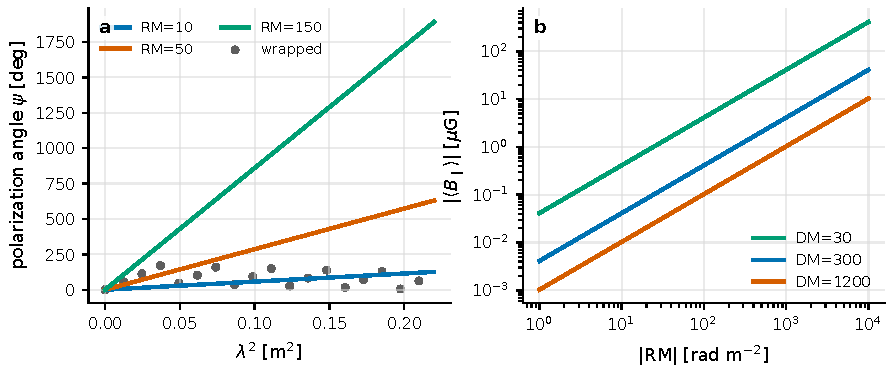
\includegraphics[width=0.94\linewidth]{figures/generated/chapter_14/ch14_faraday_rotation.pdf}
\caption{Faraday 旋转的两种读法。左图是 \(\psi=\psi_0+{\rm RM}\,\lambda^2\) 的线性关系；黑点提醒我们偏振角只能在模 \(\pi\) 意义下测得，窄带数据容易出现 \(n\pi\) 缠绕歧义（需要够宽的 \(\lambda^2\) 覆盖才能定唯一斜率）。右图把 \(\langle B_\parallel\rangle=1.232\,{\rm RM}/{\rm DM}\) 画成 RM 的函数：同一个 RM，在低 DM 的稀薄介质里代表更强的平均磁场。}
\label{fig:e21-faraday}
\end{figure}

对相干与偏振测量，Faraday 旋转的意味很直接：如果你的接收带宽跨了不小的 \(\lambda^2\) 范围，而 RM 又大，那么带宽内不同频率的偏振角被转到不同方向，把它们不加校正地平均，会\textbf{冲淡}（depolarize）净偏振——这正是第 \ref{chap:e02} 章"带宽内相位不齐会削弱相干叠加"那条精神在偏振维度上的翻版。校正的办法就是先测 RM、把每个频道的偏振角旋回本征值，再相干叠加。

\section{散射与闪烁：多路径如何搅乱相干}
\label{sec:e21-scattering}

色散和 Faraday 旋转都很"绅士"：它们只给不同频率、不同偏振加一个确定的相对延迟或旋转，去掉就还原。散射（scattering）不一样，它动的是\textbf{方向}和\textbf{相干性}本身。星际电子密度不是光滑的，湍流在各种尺度上搅出密度起伏，这些起伏像磨砂玻璃一样把平整的波前揉皱。揉皱的后果有三：源的像被角展宽（angular broadening），窄脉冲被拖出长尾（temporal broadening），强度随时间频率闪烁（scintillation）——三件事其实是同一件事在角度、时间、频率上的三个投影。

先看时间上的拖尾。波前被揉皱后，光可以走许多条稍长的路径到达我们，相当于源端一个瞬间的信号被摊到一小段时间里。在最简单的\textbf{单薄屏}（thin screen）近似下，观测脉冲是源脉冲和一个到达时间核的卷积：
\begin{equation}
  I_{\rm obs}(t)
  =
  \int I_{\rm src}(t')\,P(t-t')\,{\rm d}t',
  \qquad
  P(t)=\frac{1}{\tau_{\rm sc}}\exp\!\left(-\frac{t}{\tau_{\rm sc}}\right)H(t).
  \label{eq:e21-scattering-convolution}
\end{equation}
\begin{formulaexplain}
\(I_{\rm obs}\) 是观测强度，\(I_{\rm src}\) 是源端强度，\(P(t)\) 是散射到达时间核，\(\tau_{\rm sc}\) 是散射展宽时标，\(H(t)\) 是阶跃函数。核是\textbf{单侧}指数：光只能被绕远路而\textbf{延迟}到达，不可能提前——所以一个对称的窄脉冲，出来变成"陡升缓降"的长尾。
\end{formulaexplain}
这里 \(\tau_{\rm sc}\) 单位是秒（或毫秒），它是长尾的 \(1/e\) 衰减时间。真实视线可能有多个屏、各向异性散射、有限源尺寸，单侧指数只是最常用的低阶模型。\(\tau_{\rm sc}\) 强烈依赖频率：
\begin{equation}
  \tau_{\rm sc}\propto \nu^{-\alpha}.
  \label{eq:e21-scattering-power}
\end{equation}
\begin{formulaexplain}
\(\alpha\) 是散射的频率指数。Kolmogorov 湍流的薄屏理论给 \(\alpha\simeq4.4\)，多频脉冲星样本的经验平均更接近 \(3.9\pm0.2\)。指数这么陡，意味着往低频走，散射尾会爆炸式变长——这是低频脉冲搜索最头疼的敌人。
\end{formulaexplain}
经验上常用一条把 \(\tau_{\rm sc}\) 和 DM、频率连起来的拟合式：
\begin{equation}
  \log_{10}\!\left(\frac{\tau_{\rm sc}}{{\rm ms}}\right)
  =
  -6.46
  +0.154\log_{10}{\rm DM}
  +1.07(\log_{10}{\rm DM})^2
  -3.86\log_{10}\!\left(\frac{\nu}{\rm GHz}\right),
  \label{eq:e21-bhat-scattering}
\end{equation}
\begin{formulaexplain}
这是一条经验散射关系（DM 以 \({\rm pc\,cm^{-3}}\) 为单位），只适合做数量级预估。二次项 \((\log_{10}{\rm DM})^2\) 反映高 DM 视线穿过更多湍流；\(-3.86\log_{10}\nu\) 就是式 \eqref{eq:e21-scattering-power} 的对数版。真实视线的湍流结构会带来远超一个数量级的散布。
\end{formulaexplain}
代数字：\({\rm DM}=300\,{\rm pc\,cm^{-3}}\)、\(\nu=1.4\,{\rm GHz}\) 时它给出毫秒量级的展宽；降到 \(0.6\,{\rm GHz}\)，靠那个 \(\nu^{-3.86}\)，展宽涨到十几毫秒甚至更多。散射把毫秒脉冲拖成几十毫秒的糊团，微结构就此丢失——这是纯粹的"污染"。

现在到本章和相干性最紧要的连接。时间上的拖尾，在频率域里等价于一条\textbf{去相关带宽}（decorrelation bandwidth）\(\Delta\nu_d\)——即闪烁图样在频率上还"记得自己"的宽度：
\begin{equation}
  \tau_{\rm sc}\simeq \frac{C_1}{2\pi\,\Delta\nu_d}.
  \label{eq:e21-decorrelation-bandwidth}
\end{equation}
\begin{formulaexplain}
\(\Delta\nu_d\) 是闪烁的去相关带宽，\(C_1\) 是与几何和散射谱有关的常数（通常 \(\sim1\)）。它就是第 \ref{chap:e02} 章"时间宽度与谱宽度成反比"那条测不准关系的散射版：多路径延迟越长（\(\tau_{\rm sc}\) 大），频率上相关带宽 \(\Delta\nu_d\) 越窄。
\end{formulaexplain}
这条式子把散射对相干测量的意义讲透了。回忆第 \ref{chap:e02} 章：相干时间 \(\tau_c\simeq1/\Delta\nu\)。散射相当于给信号叠了一个额外的、随机的相位结构，它的"相干带宽"就是 \(\Delta\nu_d\)。当散射很强，\(\Delta\nu_d\) 窄得只有几十 kHz，你在一个几百 MHz 的宽带里做相干叠加，等于把几千个互不相干的斑块硬加起来——净相干度被冲淡到几乎为零。反过来，散射也\textbf{编码}信息：当散射较弱、\(\Delta\nu_d\) 可测时，闪烁斑随时间频率的漂移能反解出散射屏的速度、屏到我们的距离、乃至源的角尺寸——一台"星际闪烁望远镜"，其等效角分辨率可达微角秒，远超任何单口径望远镜。这就是散射的两副面孔：既是抹平相干的磨砂玻璃，又是免费的超高分辨探针。

\begin{figure}[tbp]
\centering
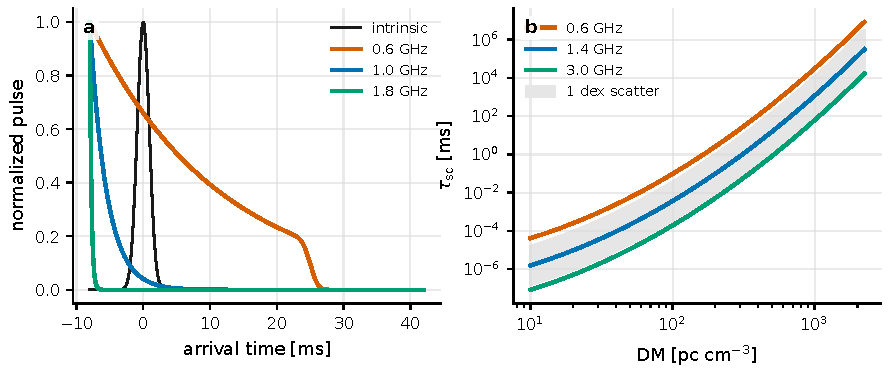
\includegraphics[width=0.94\linewidth]{figures/generated/chapter_14/ch14_scattering_broadening.pdf}
\caption{星际散射把短脉冲拖成带长尾的到达时间分布。左图把一个窄高斯脉冲与单侧指数核卷积；频率越低，\(\tau_{\rm sc}\propto\nu^{-4}\) 把尾巴拉得越长，脉冲的对称性被彻底破坏。右图用经验关系画出 \(\tau_{\rm sc}\) 随 DM 与频率的变化，灰带表示固定 DM 下常见的一个数量级以上的散布。}
\label{fig:e21-scattering}
\end{figure}

顺带一提：等离子体不只会"揉皱"波前，横向的电子柱密度梯度还能像一枚（频率相关的）透镜那样\textbf{折射}光线，低频偏折更强，可造成窄带的放大、焦散甚至多像。这提醒我们，即便把 \(\nu^{-2}\) 色散去干净了，动态谱里残留的结构也可能仍是传播的产物，而非源的本征变化 \citep{1998ApJ...496..253C,2014MNRAS.437.2180E}。在银心方向做毫米波 VLBI 时，这道强散射屏尤其麻烦：给 Sgr A* 的事件视界尺度成像，必须同时处理本征结构、散射模糊和时间变化 \citep{2008Natur.455...78D,2022ApJ...930L..14E,2022ApJ...930L..15E}。

\section{尘埃：一条带波长选择的损耗通道}
\label{sec:e21-dust}

等离子体主要动射电和到达时间；尘埃（dust）主要动光学、红外的\textbf{通量与颜色}。对光学光子，尘埃颗粒像一条挑肥拣瘦的损耗通道：它按波长选择性地吸收和散射，短波（蓝光）损失得比长波（红光）多，于是穿过尘埃的星光既变暗又变红。最基本的消光关系是
\begin{equation}
  F_{\lambda,{\rm obs}}
  =
  F_{\lambda,{\rm int}}\,10^{-0.4A_\lambda},
  \label{eq:e21-extinction-flux}
\end{equation}
\begin{formulaexplain}
\(F_{\lambda,{\rm int}}\) 是本征通量，\(F_{\lambda,{\rm obs}}\) 是消光后的通量，\(A_\lambda\) 是波长 \(\lambda\) 处的消光，单位星等（mag）。星等本就是对数标度，所以 \(A_\lambda\) 在指数上以 \(10^{-0.4A_\lambda}\) 的形式压低通量：\(A_\lambda=1\) 星等对应通量降到约 \(0.40\) 倍，\(A_\lambda=2.5\) 对应降到约 \(0.10\) 倍。
\end{formulaexplain}
消光随波长的变化，用两个量来概括其"红化"程度：
\begin{equation}
  E(B-V)=A_B-A_V,
  \qquad
  R_V=\frac{A_V}{E(B-V)}.
  \label{eq:e21-rv-definition}
\end{equation}
\begin{formulaexplain}
\(E(B-V)\) 是蓝波段 \(B\) 与可见波段 \(V\) 消光之差，叫\textbf{色余}（color excess），度量星光被"染红"了多少；\(R_V=A_V/E(B-V)\) 是总消光对选择性红化之比，度量消光曲线的"灰度"。\(R_V\) 越大，曲线越平（越灰），说明较大的尘埃颗粒占主导。
\end{formulaexplain}
逐项落地：\(A_B,A_V\) 是 \(B\)、\(V\) 波段的消光（各以 mag 计），\(E(B-V)\) 单位也是 mag。银河系平均 \(R_V\simeq3.1\)，弥散星际介质多在 \(2.5\text{--}3.5\)，致密分子云里可到 \(5\) 以上（大颗粒使消光更灰）。Cardelli–Clayton–Mathis（CCM）消光律把红外、光学、紫外的平均曲线压缩成一个由 \(R_V\) 参数化的单参数族；Fitzpatrick 进一步指出真实视线仍有明显散布，尤其在 \(2175\,\text{\AA}\) 的紫外驼峰（UV bump）和远紫外上翘的强弱上 \citep{1989ApJ...345..245C,1999PASP..111...63F,2003ARA&A..41..241D}。

这里有一个对瞬变和偏振测量至关重要的\textbf{误差地板}。若你只用一条平均消光律去改正一个 \(E(B-V)=0.2\) 星等的蓝色源，紫外端残留 \(0.1\) 星等的误差毫不稀奇——对偏振角、颜色温度、以及瞬变源早期的谱能量分布（SED），这就是主导性的系统误差。换句话说，尘埃不仅让源变暗，它还给"颜色"这个测量注入了不可忽视的不确定度。

尘埃颗粒多是非球形的，它们在星际磁场里会部分排列取向，于是对不同振动方向的星光吸收不等，给穿过的星光注入一点\textbf{线偏振}。其波长依赖用经验的 Serkowski 关系描述：
\begin{equation}
  \frac{P(\lambda)}{P_{\max}}
  =
  \exp\!\left[-K\ln^2\!\left(\frac{\lambda_{\max}}{\lambda}\right)\right].
  \label{eq:e21-serkowski}
\end{equation}
\begin{formulaexplain}
\(P(\lambda)\) 是尘埃造成的线偏振度，\(P_{\max}\) 是峰值偏振，\(\lambda_{\max}\) 是峰值波长，\(K\) 控制曲线宽度。它是一条以 \(\ln(\lambda_{\max}/\lambda)\) 为变量的高斯型峰：偏振在 \(\lambda_{\max}\) 处最大，向两侧对称衰减。峰的位置 \(\lambda_{\max}\) 对颗粒尺寸敏感。
\end{formulaexplain}
经验上 \(\lambda_{\max}\approx0.55\,\mu{\rm m}\)，峰值偏振度的上限约为 \(P_{\max}\lesssim9\,E(B-V)\%\)（即每 0.1 mag 色余最多约 0.9\% 偏振）。这个上限并非每条视线都能达到，它受颗粒形状、取向效率、视线上磁场方向的变化、以及多层云叠加影响 \citep{1975ApJ...196..261S,2015ARA&A..53..501A}。对任何想测源本征偏振的实验，这条尘埃偏振是必须先扣掉的前景。

尘埃还能把一次短暂的爆发"回放"成\textbf{光回声}（light echo）或 X 射线晕：爆发的光被途中尘埃散射进我们的视线，因为绕了个弯，比直达光晚到。若尘埃屏位于源到观测者距离的比例 \(x\) 处、散射角为 \(\theta\)，几何延迟近似为
\begin{equation}
  \Delta t_{\rm dust}
  \simeq
  \frac{D_s}{2c}\,\frac{x}{1-x}\,\theta^2 .
  \label{eq:e21-dust-delay}
\end{equation}
\begin{formulaexplain}
\(\Delta t_{\rm dust}\) 是尘埃散射的几何延迟，\(D_s\) 是源距离，\(x\) 是尘埃屏的相对位置（\(0\) 在源、\(1\) 在观测者），\(\theta\) 是散射角。延迟正比于 \(\theta^2\)，所以角分辨的光回声能反推尘埃的几何位置——延迟随散射角的展开，就是一把测距的尺。
\end{formulaexplain}
数量级上，对银河系源，角秒级散射角给出小时到天的延迟；对河外源，尘埃的几何位置和望远镜角分辨要一起进入模型。这又是一次"污染即编码"：本来是挡光的尘埃，借着延迟–角度关系，成了测量爆发周围三维尘埃分布的探针。

\begin{figure}[tbp]
\centering
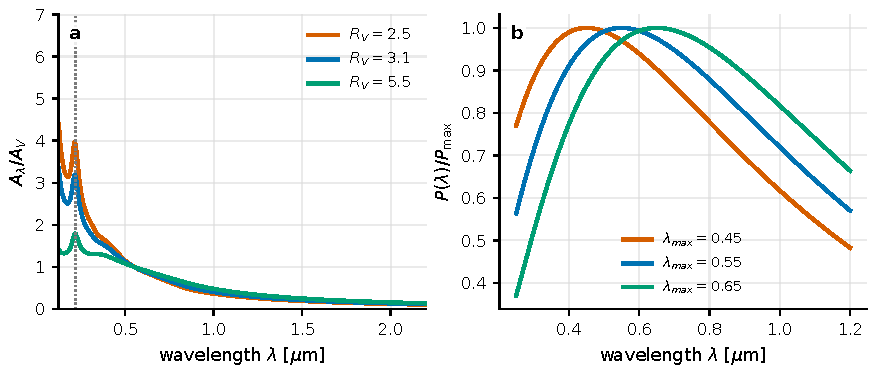
\includegraphics[width=0.94\linewidth]{figures/generated/chapter_14/ch14_dust_extinction_polarization.pdf}
\caption{尘埃同时改变光子的通量、颜色与偏振。左图是 CCM 平均消光曲线，\(R_V\) 越大、光学到近红外越"灰"；\(0.2175\,\mu{\rm m}\) 附近的紫外驼峰是小颗粒和碳质材料的重要诊断。右图是 Serkowski 偏振曲线，峰位 \(\lambda_{\max}\) 的移动反映颗粒尺寸与取向环境的变化。}
\label{fig:e21-dust}
\end{figure}

\section{引力透镜：把一条路径变成多条}
\label{sec:e21-lensing}

前面三位改写者都来自真实的介质——电子、磁场、尘埃颗粒。最后一位不一样：引力透镜（gravitational lensing）来自\textbf{弯曲的时空}本身。它不改变光子的频率（不色散），却改变光走的路径、方向和到达时间。对事件表来说，透镜的核心动作可以用一句话概括：\textbf{一个源事件，可以变成多个像、多个到达时刻、多个放大权重}。

在薄透镜近似下，源的真实方向和我们看到的像方向由透镜方程连接：
\begin{equation}
  {\boldsymbol\beta}
  =
  {\boldsymbol\theta}
  -
  {\boldsymbol\alpha}({\boldsymbol\theta}),
  \label{eq:e21-lens-equation}
\end{equation}
\begin{formulaexplain}
\({\boldsymbol\beta}\) 是源的真实角位置，\({\boldsymbol\theta}\) 是像的角位置，\({\boldsymbol\alpha}\) 是约化偏折角（reduced deflection angle），都以角度（rad 或 arcsec）计。方程说：我们看到的像方向 \({\boldsymbol\theta}\)，等于真实方向 \({\boldsymbol\beta}\) 加上质量把光线扳过来的角度。给定 \({\boldsymbol\beta}\)，这个方程可以有\textbf{多个} \({\boldsymbol\theta}\) 解——那就是多重像。
\end{formulaexplain}
偏折的自然角尺度由 Einstein 角给出。对一个点质量透镜，
\begin{equation}
  \theta_E
  =
  \left(
  \frac{4GM}{c^2}
  \frac{D_{ls}}{D_lD_s}
  \right)^{1/2}.
  \label{eq:e21-einstein-angle}
\end{equation}
\begin{formulaexplain}
\(\theta_E\) 是 Einstein 角，\(M\) 是透镜质量，\(G\) 是引力常数，\(D_l,D_s,D_{ls}\) 分别是观测者到透镜、到源、以及透镜到源的角直径距离。核心因子 \(4GM/c^2\) 就是广义相对论光线偏折的招牌（是牛顿预言的两倍）。\(\theta_E\) 定下多重像分离与微透镜的天然尺度。
\end{formulaexplain}
两个真实数量级把两种透镜分开。\(M=1\,M_\odot\)、银河系尺度几何，给出毫角秒（mas）量级的 \(\theta_E\)——这么小分不开两个像，只能看到亮度随时间起伏，这就是\textbf{微透镜}（microlensing）：一颗前景恒星飘过背景星前面，把它短暂放大。而 \(M\sim10^{11}\text{--}10^{12}\,M_\odot\) 的星系透镜，给出角秒（arcsec）量级的 \(\theta_E\)，多重像清清楚楚分得开，这是\textbf{强透镜}（strong lensing）。放大率由像面到源面的映射的雅可比行列式决定：
\begin{equation}
  \mu
  =
  \frac{1}{\det\!\left(\partial{\boldsymbol\beta}/\partial{\boldsymbol\theta}\right)}.
  \label{eq:e21-magnification}
\end{equation}
\begin{formulaexplain}
\(\mu\) 是放大率，分母是从像平面 \({\boldsymbol\theta}\) 到源平面 \({\boldsymbol\beta}\) 的雅可比行列式。透镜不产生也不吸收光子，只是重新分配立体角，所以面积被拉伸多少倍，亮度就放大多少倍。当行列式趋于零，像面被无限拉伸，放大率发散——那条曲线叫焦散（caustic）。
\end{formulaexplain}
焦散附近 \(|\mu|\) 可以非常大（理论上发散），但有限的源尺寸、微透镜、尘埃和时间采样都会把实际能观测到的峰值放大压下来。这条式子的物理很干净：放大是几何的重新分配，不是能量的凭空增加。

现在到透镜最深刻、也最贴合本书主线的一点：\textbf{时间延迟}。不同的像走的是不同长度、且穿过不同深浅引力势的路径，所以它们的光不是同时到达的。到达时间由 Fermat 势（Fermat potential）控制：
\begin{equation}
  t({\boldsymbol\theta},{\boldsymbol\beta})
  =
  \frac{D_{\Delta t}}{c}
  \left[
  \frac{1}{2}\,|{\boldsymbol\theta}-{\boldsymbol\beta}|^2
  -
  \psi({\boldsymbol\theta})
  \right],
  \qquad
  D_{\Delta t}
  =
  (1+z_l)\frac{D_lD_s}{D_{ls}} .
  \label{eq:e21-fermat-delay}
\end{equation}
\begin{formulaexplain}
\(t\) 是相对到达时间，方括号里第一项 \(\tfrac12|{\boldsymbol\theta}-{\boldsymbol\beta}|^2\) 是\textbf{几何路径差}（绕远路多花的时间），第二项 \(\psi\) 是\textbf{引力势延迟}（Shapiro 延迟，光在深势阱里"走得慢"）。\(D_{\Delta t}\) 是时间延迟距离，\(z_l\) 是透镜红移。真实的像出现在这个时间面的\textbf{驻点}（极小、极大或鞍点）——这正是费马原理："光走极值时间的路"。
\end{formulaexplain}
时间延迟的几何起源就藏在这两项的拉锯里：偏离源方向越远，几何项越大（迟到），但通常也越靠近质量、势阱越深（Shapiro 项也在变）。两幅像的观测延迟，就是它们 Fermat 势之差：
\begin{equation}
  \Delta t_{AB}
  =
  \frac{D_{\Delta t}}{c}\,
  \Delta\phi_{AB}.
  \label{eq:e21-time-delay-distance}
\end{equation}
\begin{formulaexplain}
\(\Delta t_{AB}\) 是像 \(A\) 与像 \(B\) 的到达时差，\(\Delta\phi_{AB}\) 是二者的 Fermat 势差（由透镜质量模型算出）。测出 \(\Delta t_{AB}\)、再有一个透镜模型给出 \(\Delta\phi_{AB}\)，就能反解出 \(D_{\Delta t}\)——而 \(D_{\Delta t}\propto 1/H_0\)，于是时间延迟直接测量了哈勃常数。
\end{formulaexplain}
数量级：星系强透镜的 \(\Delta t_{AB}\) 常为天到月，少数可达年。注意它只占 \(D_{\Delta t}/c\) 的约 \(10^{-11}\)（因为 \(\Delta\phi_{AB}\) 是个小数），所以透镜势、外部收敛（external convergence）、质量片简并（mass-sheet degeneracy）和光变曲线采样的每一点误差，都会直接灌进 \(H_0\) 的误差预算。Refsdal 早在 1964 年就指出多重像时间延迟可以测 \(H_0\)；现代的时间延迟宇宙学（time-delay cosmography）靠多年监测、高分辨成像、透镜星系速度弥散和环境建模，把这条思路做成了独立于宇宙微波背景的 \(H_0\) 测量 \citep{1964MNRAS.128..295R,1964MNRAS.128..307R,1986ApJ...310..568B,2016A&ARv..24...11T}。这是本章的又一记漂亮编码：时间延迟本是"同一个源被复制出好几个错时副本"的污染，结果这错时里锁着宇宙的膨胀率。

\begin{figure}[tbp]
\centering
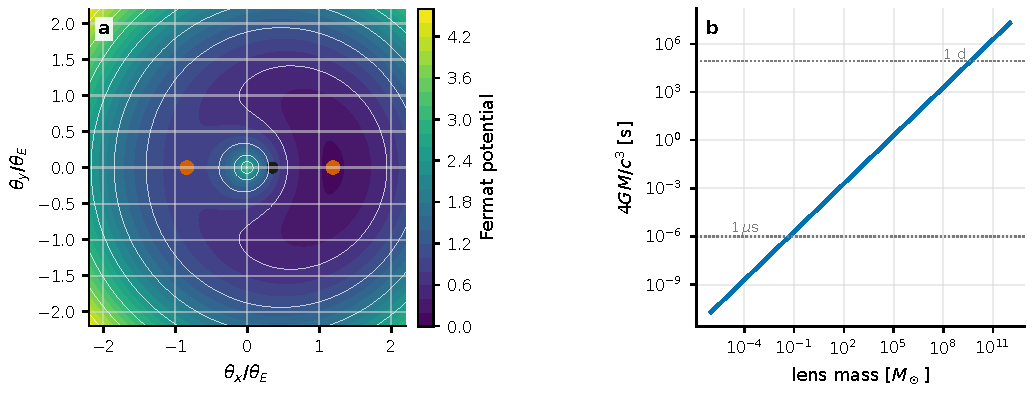
\includegraphics[width=0.94\linewidth]{figures/generated/chapter_14/ch14_lensing_time_delay.pdf}
\caption{强透镜的两个尺度。左图是点质量透镜的 Fermat 到达时间面，黑点是源位置，两个橙点是像位置；像恰好出现在到达时间面的驻点（极小与鞍点）。右图给出基本延迟尺度 \(4GM/c^3\)：恒星质量透镜落在微秒到毫秒，星系与星系团透镜自然进入天到年的时间域。}
\label{fig:e21-lensing}
\end{figure}

\paragraph{当波长不能忽略：从光线到衍射}
\label{sec:e21-wavelensing}

前面把光当成"光线"，默认多条路径可以清清楚楚分开。但当波长和透镜引起的时间延迟相当时，几何光学失效，必须回到\textbf{波}的图像——就像第 \ref{chap:e02} 章反复强调的，波会衍射、会干涉。判据是一个无量纲频率：
\begin{equation}
  w
  =
  \frac{8\pi GM(1+z_l)f}{c^3}.
  \label{eq:e21-wave-lensing-w}
\end{equation}
\begin{formulaexplain}
\(w\) 是波动透镜的无量纲频率，\(M\) 是透镜质量，\(f\) 是波的频率，\(z_l\) 是透镜红移。\(w\) 比较的是波的周期 \(1/f\) 与透镜引起的时间延迟尺度 \(\sim GM/c^3\)：\(w\gg1\) 时延迟远长于周期，回到几何光学；\(w\lesssim1\) 时延迟不到一个周期，衍射不可忽略。
\end{formulaexplain}
在几何区（\(w\gg1\)），多重像可以分开，并像双缝一样相干干涉；在衍射区（\(w\lesssim1\)），焦散被抹平，放大率不再能简单地把几何像相加。频域波形写成
\begin{equation}
  \tilde h_L(f)=F(f)\,\tilde h(f),
  \label{eq:e21-wave-amplification}
\end{equation}
\begin{formulaexplain}
\(\tilde h(f)\) 是未透镜的频域波形，\(\tilde h_L(f)\) 是透镜后的，\(F(f)\) 是复放大因子（complex amplification factor）。它是复数，所以同时携带\textbf{振幅放大}（模）和\textbf{相位延迟}（辐角），能造出频率依赖的干涉花纹。
\end{formulaexplain}
若两条路径延迟为 \(\Delta t\)，两路复振幅相加，随频率的拍频给出频域条纹间隔
\begin{equation}
  \Delta f \simeq \frac{1}{\Delta t}.
  \label{eq:e21-lensing-fringe-spacing}
\end{equation}
\begin{formulaexplain}
\(\Delta f\) 是频域干涉条纹的间距，\(\Delta t\) 是两条路径的时间延迟。这正是傅里叶那条老规矩（第 \ref{chap:e02} 章）的又一次现身：时间上相隔 \(\Delta t\) 的两个副本，在频谱上织出间距 \(1/\Delta t\) 的条纹。路径延迟越长，频域振荡越密。
\end{formulaexplain}
代数字：\(\Delta t=2\,{\rm ms}\) 给出 \(\Delta f\approx500\,{\rm Hz}\) 的条纹间隔。对光学、射电的电磁波频率 \(f\sim10^{14}\) 或 \(10^{9}\,{\rm Hz}\)，普通恒星或星系质量透镜的 \(w\) 大得惊人，几何光学好得几乎完美；但对 LISA 频段的引力波（\(f\sim10^{-3}\,{\rm Hz}\)）配上 \(10^{6}\text{--}10^{9}\,M_\odot\) 的透镜，\(w\sim1\) 的波动光学效应会真的落进观测带 \citep{2003ApJ...595.1039T}。这是透镜与本书量子光学主线最直接的接口：透镜后的干涉，本质上是同一个源场沿两条路径的相干叠加，读的还是相位。

\begin{figure}[tbp]
\centering
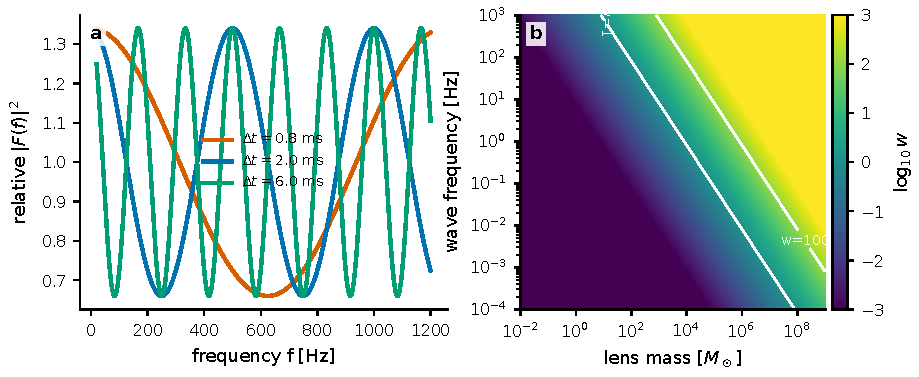
\includegraphics[width=0.94\linewidth]{figures/generated/chapter_14/ch14_wave_lensing_interference.pdf}
\caption{波动光学透镜把时间延迟转写成频域条纹。左图画出不同路径延迟下相对放大因子的振荡，条纹间距 \(\Delta f\simeq1/\Delta t\)。右图给出 \(w=8\pi GMf/c^3\) 的量级；白线 \(w=1\) 附近是衍射与几何光学的过渡，\(w\gtrsim100\) 时通常可把各像当成独立路径处理。}
\label{fig:e21-wave-lensing}
\end{figure}

\section{污染还是编码：传播对相干与计时的意义}
\label{sec:e21-correlation}

绕了一圈，回到本书的主线——相关函数。前面几节都在改写\textbf{单个事件的标签}，这一节要看它们如何改写\textbf{事件之间的相关}。核心洞见很简单：多路径传播（散射、透镜）会重排强度相关，因为观测到的两次涨落，未必来自源端同一时刻——它们可能是源端同一个结构沿不同路径、错时到达的两个副本。

把可分辨的多路径写成一串 delta 脉冲响应：
\begin{equation}
  h(t)=\sum_i \sqrt{\mu_i}\,e^{i\varphi_i}\,\delta(t-t_i),
  \label{eq:e21-multipath-impulse}
\end{equation}
\begin{formulaexplain}
\(h(t)\) 是多路径脉冲响应，\(\mu_i\) 是第 \(i\) 条路径的放大率，\(\varphi_i\) 是它的相位，\(t_i\) 是它的到达延迟。每个 delta 函数就是一条可分辨的路径——它是式 \eqref{eq:e21-channel-time} 那个抽象 \(h_{ij}\) 在"离散多像"情形下的具体样子。
\end{formulaexplain}
如果相位 \(\varphi_i\) 在观测带宽或源尺寸上被平均掉（相干被冲淡时的常见情形），观测强度就是各路径强度按放大率加权、错时叠加：
\begin{equation}
  I_{\rm obs}(t)
  =
  \sum_i \mu_i\,I_{\rm src}(t-t_i).
  \label{eq:e21-multipath-intensity}
\end{equation}
\begin{formulaexplain}
\(I_{\rm obs}\) 是观测强度，\(I_{\rm src}\) 是源端强度。相位平均后，干涉项消失，只剩各路径的强度按 \(\mu_i\) 加权相加——所以源端的一次变化，会在几个不同延迟 \(t_i\) 处各重复一遍。
\end{formulaexplain}
对强度涨落 \(\delta I=I-\langle I\rangle\) 做自相关，就能看到"回声"如何进入相关函数：
\begin{equation}
  C_{\rm obs}(\tau)
  =
  \left\langle
  \delta I_{\rm obs}(t)\,
  \delta I_{\rm obs}(t+\tau)
  \right\rangle
  =
  \sum_{ij}\mu_i\mu_j\,
  C_{\rm src}\!\left(\tau+t_i-t_j\right).
  \label{eq:e21-correlation-echo}
\end{equation}
\begin{formulaexplain}
\(C_{\rm obs}\) 是观测强度自相关，\(C_{\rm src}\) 是源端自相关。双重求和意味着\textbf{每一对路径}都贡献一个相关回声，回声出现在 \(\tau=t_j-t_i\) 处，权重是 \(\mu_i\mu_j\)。原本一个峰，被复制成一梳子的回声峰。
\end{formulaexplain}
这条式子把传播对第 \ref{chap:e08} 章那套强度相关工具的影响说清楚了：\textbf{相关峰不再唯一对应源端物理}。热光的 \(g^{(2)}(0)\) 峰、脉冲星巨脉冲的微结构、FRB 的窄带闪烁、透镜多像的延迟，都能落进这个框架，但它们的相干时间、带宽和统计分布各不相同——光看到一个相关峰，还不足以断定它的物理来源。用式 \eqref{eq:e21-correlation-echo} 时的前提很硬：源本身要有可测的快结构、传播路径要稳定、观测时间要够长、背景与选择函数要建过模。这正是把传播当成"有记忆通道"这个视角的回报——它逼你在解读任何相关峰之前，先问一句"这会不会只是一条晚到的路径？"

传播效应还划定了一类量子基础实验的边界。所谓宇宙 Bell 检验（cosmic Bell test），用纠缠光子对在两个站点做测量，两边各选测量设置 \(a,a'\) 和 \(b,b'\)，构造 CHSH 组合：
\begin{equation}
  S
  =
  E(a,b)+E(a,b')+E(a',b)-E(a',b'),
  \qquad
  |S|\le 2 .
  \label{eq:e21-chsh}
\end{equation}
\begin{formulaexplain}
\(S\) 是 CHSH 组合，\(E(a,b)\) 是给定设置下两站测量结果的相关期望值。局域隐变量理论要求 \(|S|\le2\)；量子力学可以违反到 \(2\sqrt2\)。宇宙 Bell 实验的独到之处，是用\textbf{天文光子}实时决定设置 \(a,b\)。
\end{formulaexplain}
它的用意不是说天体光子本身处于纠缠态，而是拿遥远天体的光子来\textbf{实时选择}测量设置：银河系恒星版本用星光颜色产生 \(a,b\)，把可能的"共同原因"推到几百到几千年前；类星体版本更狠，把自由选择漏洞的共同过去推到宇宙早期 \citep{2017PhRvL.118f0401H,2018PhRvL.121h0403R}（图 \ref{fig:e21-cosmic-bell}）。而这正需要本章全部内容：星光的到达时间要扣掉大气延迟（第 \ref{chap:e13} 章的时间同步），颜色要扣掉尘埃红化，射电类星体还要考虑色散和散射，仪器电子延迟要逐项进入实验时序——传播中的每一项吸收、红化、色散、延迟，都必须放进实验的因果时序里，否则漏洞就补不严。

\begin{figure}[tbp]
\centering
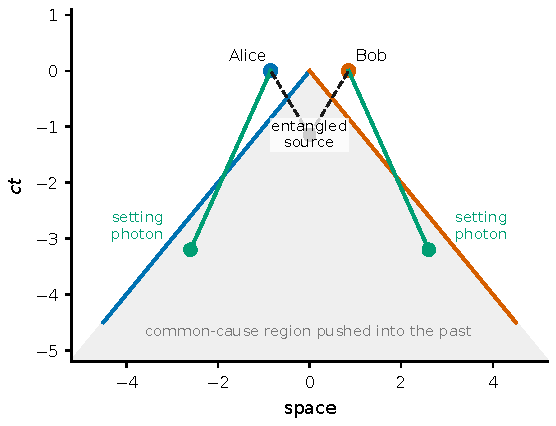
\includegraphics[width=0.72\linewidth]{figures/generated/chapter_14/ch14_cosmic_bell_lightcones.pdf}
\caption{宇宙 Bell 实验的光锥结构。纠缠源在本地实验中发出光子对，Alice 与 Bob 的测量设置由远处恒星或类星体的光子实时决定；这些设置光子的发射事件越早、方向分离越大，能被排除掉"共同原因"的时空区域就越大（图中灰区）。真实实验还要逐项加入大气传播、尘埃红化、探测器响应与电子延迟——这正是本章各效应必须进入实验时序的地方。}
\label{fig:e21-cosmic-bell}
\end{figure}

最后，把这些"平常的"传播效应看成新物理搜索的\textbf{误差地板}。类轴子粒子（axion-like particle）可以让光子在磁场里转化而造成谱吸收，宇宙双折射会旋转偏振，暗物质小结构能改写透镜的放大率和时间延迟——这些迷人的解释，都必须先和等离子体色散、尘埃、常规透镜、仪器项放在同一个模型里比较。只有当一个残余信号同时经得起时间、频率、偏振、角位置四道检验、且已知传播效应都扣不掉它时，它才有资格排队当新物理的候选。这就是"污染即背景，编码即信号"这条本章主旨最实用的收尾：先把这条有记忆的通道刻画到底，剩下的才是真正属于源、乃至属于新物理的东西。

\section*{本章要点}
\addcontentsline{toc}{section}{本章要点}

\begin{itemize}
\item \textbf{传播是有记忆的通道，不是灰玻璃。} 式 \eqref{eq:e21-channel-time} 把源端场到探测器事件写成卷积：介质重写每个光子的时间、频率、偏振、方向标签，而不只是乘一个常数。
\item \textbf{色散的 \(\nu^{-2}\) 定律是从群速度一步步推出来的。} 折射率 \(\to\) 群速度 \(v_g\approx c(1-\omega_p^2/2\omega^2)\) \(\to\) 沿视线积分，得到 \(\Delta t\propto{\rm DM}/\nu^2\)（式 \eqref{eq:e21-dm-delay}）。低频迟到的根源就是"低频群速度更慢"。DM 是电子柱密度，FRB 的 DM–红移关系能称量宇宙重子。
\item \textbf{Faraday 旋转给色散补上磁场方向。} 偏振角对 \(\lambda^2\) 的斜率是 RM，它的被积函数 \(n_e B_\parallel\) 带符号，故 RM/DM 给出电子加权平均磁场（式 \eqref{eq:e21-bfield-rm-dm}），但仅当二者同源才有直接物理含义。
\item \textbf{散射搅乱相干，也免费提供超高分辨。} 单侧指数核把窄脉冲拖成长尾（\(\tau_{\rm sc}\propto\nu^{-4}\)），去相关带宽 \(\Delta\nu_d\simeq1/2\pi\tau_{\rm sc}\)（式 \eqref{eq:e21-decorrelation-bandwidth}）决定宽带相干叠加会不会被冲淡；弱散射时闪烁反能反解屏速度、屏距离与源角尺寸。
\item \textbf{尘埃是带波长选择的损耗通道。} 消光 \(F_{\rm obs}=F_{\rm int}10^{-0.4A_\lambda}\) 让源既暗又红，\(R_V\) 定曲线灰度；平均消光律的残差是偏振与早期 SED 的主导系统误差；Serkowski 偏振和尘埃光回声都是必须先扣的前景。
\item \textbf{引力透镜把一条路径变成多条。} Einstein 角定尺度（恒星质量 mas，星系 arcsec），放大率是几何雅可比的倒数，时间延迟由 Fermat 势的几何项加 Shapiro 项决定（式 \eqref{eq:e21-fermat-delay}），并因 \(D_{\Delta t}\propto1/H_0\) 而测量哈勃常数。波长不可忽略时用无量纲频率 \(w\) 判几何/衍射区。
\item \textbf{污染即编码。} 多路径把源端一次涨落复制成相关回声（式 \eqref{eq:e21-correlation-echo}），所以相关峰不唯一对应源端物理；这些常规效应又构成宇宙 Bell 检验的时序约束与新物理搜索的误差地板。
\end{itemize}

\medskip
\noindent\textbf{想一想。}
\begin{itemize}
\item 若某 FRB 在 \(1.4\,{\rm GHz}\) 和 \(0.8\,{\rm GHz}\) 之间测得 \(1.2\,{\rm s}\) 的延迟，它的 DM 约是多少？（用式 \eqref{eq:e21-dispersion-delay} 反解。）这条视线若主要在银河系内，对照高银纬典型值合理吗？
\item 同样一个 RM，如果视线上存在一次磁场反向，你测到的 RM 会偏大还是偏小？为什么 DM 不受这个反向影响？
\item 一个星系强透镜的两幅像时间延迟测得 \(30\) 天，透镜模型给出 \(\Delta\phi_{AB}\)。要把 \(H_0\) 测到 3\% 精度，式 \eqref{eq:e21-time-delay-distance} 里哪些环节（光变采样、外部收敛、质量片简并）最可能成为瓶颈？
\end{itemize}
